\documentclass[parskip]{komatufte}
\usepackage[subpreambles=false]{standalone}

%%%%%%%%%%%%%%%%%%%%%%%%%%%
% Silence warning messages
\usepackage{silence}
\WarningsOff[scrlayer-notecolumn]
\WarningsOff[biblatex]

%%%%%%%%%%%%%%%%%%%%
% Commenting

%\usepackage[author=Lyndon]{pdfcomment}
%\newcommand{\pdfcomment}[1]{} %ignore all comments

%\usepackage{todonotes}
%\newcommand{\pdfcomment}{\todo}


%%%%%%%%%%%%%%%%%%%%
% Tables
\usepackage{booktabs}

%%%%%%%%%%%%%%%%%%%
% Fonts
\usepackage{tgadventor} %sans
\usepackage{tgpagella}  %serif
\usepackage{inconsolata} %mono
\usepackage[T1]{fontenc}

\usepackage{microtype}
\usepackage[all]{nowidow}
%%%%%%%%%%%%%%%%%%%%%%%
% Styling
\setcounter{secnumdepth}{4}
\setcounter{tocdepth}{2}

\usepackage{placeins}



%%%%%%%%%%%%%%%%%%%
% Math
\usepackage{amsmath, amssymb, stmaryrd, mathtools}
\DeclareMathOperator*{\argmin}{argmin}
\DeclareMathOperator*{\argmax}{argmax}

\usepackage{xparse,xstring,etoolbox}
% crossref this against notation section
\newcommand{\vv}[1]{\tilde{#1}} % vector
\newcommand{\seq}[1]{\mathcal{#1}} % sequence
\newcommand{\set}[1]{\mathbb{#1}} % set

%%%%%%%%%
% Indexing/sequence indexing
\newcommand{\seqind}[2]{#1^{#2}} % seqence index
\newcommand{\ind}[2]{#1_{#2}} % indexed
\newcommand{\disamb}[2]{#1^{\mathrm{#2}}} %disambiguated

%% Smart indexing and naming
\newcommand{\ifupper}[3]{
    \normalexpandarg
	\exploregroups
	\StrCount{ABCDEFGHIJKLMNOPQRSTUVWXYZ}{#1}[\uppercount]
	\ifnumgreater{\uppercount}{0}{#2}{#3}
}

%smart index
\DeclareDocumentCommand{\ii}{u{_} m}{
	\ifupper{#1}%
	{% just a single uppercase character, i.e. a matrix
		  %make sure the index is the right length
		\StrCount{#2}{,}[\indcount]
		\ifnumgreater{\indcount}{0}
		{ % Got multiple indexes so all good
		 	\ind{#1}{#2}
		}
		{ % Only 1 index so grab the column
		 	\ind{#1}{{:,#2}}
		}
	}%
	{% Not just a single upper case character
		\ind{#1}{#2}
	}
}

\DeclareDocumentCommand{\nn}{u{_} m}{
	\seqind{#1}{#2}
}

\DeclareDocumentCommand{\dd}{u{_} m}{
	\disamb{#1}{#2}
}

% Index of a vector
\DeclareDocumentCommand{\iv}{u{_} m}{\ii{\vv #1}_{#2}}
\DeclareDocumentCommand{\dv}{u{_} m}{\dd{\vv #1}_{#2}}
\DeclareDocumentCommand{\nv}{u{_} m}{\nn{\vv #1}_{#2}}

%exp
\let\oldexp\exp
\renewcommand{\exp}[1]{\oldexp \left( #1 \right)}
\newcommand{\exptwo}[1]{\oldexp_2 \left( #1 \right)}

\newcommand{\softmax}{\mathrm{smax}}

\DeclareMathOperator*{\expectedop}{\mathbb{E}}
\DeclareDocumentCommand{\expected}{u{_} m}{
	\expectedop\limits_{\mathrlap{#2}}
}

%%%%%%%%%%%%%%%%
%Graphics
\usepackage{tikz}
\usetikzlibrary{positioning, fit,  shapes.geometric}
\usepackage{ifthen}
\usepackage{etoolbox}

\tikzset{
	backgroundcolor/.style ={fill=white},
	every node/.append style={
		minimum height=7mm,
	},
	labe/.append style={
		%Blue,
		align = center,
		backgroundcolor,
		fill opacity=0.6,
		text opacity=1,
		font={\footnotesize\itshape}	
	},
	layer/.append style={
		draw,
		align = center,
		minimum height=7mm,
	},
	tight/.append style={
		inner sep=0.2mm,
	},
	lookupbox/.append style={
		draw=none,
		append after command={
		       	[shorten <= -0.5\pgflinewidth]
		       	([shift={(-1.5\pgflinewidth,-0.5\pgflinewidth)}]\tikzlastnode.north east)
		       	edge([shift={( 0.5\pgflinewidth,-0.5\pgflinewidth)}]\tikzlastnode.north west) 
		       	([shift={( 0.5\pgflinewidth,-0.5\pgflinewidth)}]\tikzlastnode.north west)
		       	edge([shift={( 0.5\pgflinewidth,-1.5\pgflinewidth)}]\tikzlastnode.south west)            
		       	([shift={( -1.5\pgflinewidth,+0.5\pgflinewidth)}]\tikzlastnode.south east)
		       	edge([shift={(-1.5\pgflinewidth,-0.5\pgflinewidth)}]\tikzlastnode.north east)
		},
		inner sep=0.7mm,
		outer sep=0mm,
		minimum width=25mm
	}
}

\usepackage{pgfplots}
\pgfplotsset{compat=1.14}
\pgfplotsset{sideplot/.append style={
		width=\notescolwidth,
		domain=-10:10,
		samples=101,
		smooth,
		enlarge y limits={abs=2},
		axis lines=middle,
		xlabel  = $z$,
		ylabel  = $y$,
	},
	equ/.append style={
		color=blue,
		thick,
		mark=none
	}
}

% Function  For a plot 
% it  needs to be declared in preamble because of how \makenote* interacts with multiple files
\def\errorsurface(#1,#2){(0.5*#1 + 0.7*#2 + sin(deg(1.5*#1 + #2^2)))^2}


\usepackage{graphicx}
\graphicspath{{./figs/}, {./}, {./figs/chaptersentencerrepr/}, {./figs/chapterintromachinelearning/}, {./figs/chapterwordrepr/}}
\usepackage{adjustbox}


%%%%%%%%%%%%%%%%%%%
% Refs
\usepackage{cleveref}

\addbibresource{master.bib}

%%%%%%%%%%%%%%%%%%%%
% Formatting

% for examples from natural language space.
\newcommand{\natlang}[1]{\ifmmode \text{``\texttt{#1}''} \else {``\texttt{#1}''}\fi}
% \ifmmode ``trick'' from https://tex.stackexchange.com/a/15194/5834

%%%%%%%%%%%%%%%%%%%%%


\graphicspath{{./figs/chapterwordrepr}, {./}}


\begin{document}
\chapter{Word Representations}\label{sec:word-representations}
\begin{abstract}
The core work that began to draw a lot of attention to this area.
This will cover crucial works such as skip-grams, CBOW, and of course the original neural probabilistic language model.
As well as the links to traditional matrix factorisations.
\end{abstract}

\aside[Word Vector or Word Embedding?]{In some older literature in the area will use the term \emph{word~vector} to refer to representations from LDA and LSA etc. Whereas in a lot of newer work the term is used synonymously with \emph{word~embedding}.}
We begin the consideration of the representation of words using neural networks with work on language modeling
This is not the only place one could begin the consideration: the information retrieval (IR) models such as LSA \pcite{dumais1988using} and LDA \pcite{blei2003latent} based on word co-location with documents would be the other obvious starting point.
However, as will be discussed there models are closer to the end point of of the chapter than the begin.
For the language modeling works, comes the contextual language model works such as skip-gram, which in turn lead to the post-neural network co-occurrence based works.
These model fundamentally are in fact more similar to the information retrieval co-location works than the language modeling from which we began.


\section{Representations for Language Modeling}

\aside[Random Variable Naming Convention]{We follow convention that capitalised $W_i$ is a random variable, and $w_i$ is a particular value which $W_i$ may take. Writing $P(\ldots W_i{=}w_i)$.
	Often though we will make uses of the abridged (abuse-of) notation and simply write $P(\ldots w_i)$, allowing the random variable to be implicitly given by the name of its value.
}

The language modeling task it to predict the next word given the words that came prior \pcite{rosenfeld2000two}.
For example, if a sentence begins \natlang{For lunch I will have a hot}, then there is a high probability that the next word will be \natlang{dog} or \natlang{meal},
and lower probabilities of words such as \natlang{day} or \natlang{are}.
Mathematically it is formulated: 
\begin{equation}\label{equ:langmodel}
	P(W_n{=}w_i \mid W_{i-1}{=}w_{i-1}, \ldots, W_1{=}w_1)
\end{equation}
or to use the compact notation 
\begin{equation}\label{equ:langmodelcompact}
P(w_i \mid w_{i-1}, \ldots, w_1)
\end{equation}
$P(w_i \mid \natlang{hot}, \natlang{a}, \natlang{want}, \natlang{I}, \natlang{lunch}, \natlang{For})$.
The task is to find the probabilities for the various words that $w_i$ could represent.

\aside[Google n-gram corpora]{Google has created several very large scale corpora of 1,2,3,4, and 5-grams from over $10^{11}$ words.
Including the 2006 Web corpus from the public internet (Available for fee at \url{https://catalog.ldc.upenn.edu/LDC2006T13}),
and the 2010-2012 Books corpus made words from the Google Books project (available freely from \url{https://books.google.com/ngrams/datasets}), as described in \textcite{lin2012syntactic}.
These very large corpora also used outside of statistical language modeling by corpus linguists investigating the use of language.
}

  
The classical approach is trigram statistical language modeling.
In this, the number of word triples in a corpus is counted,
then given the previous two words, the next is predicted based on those counts.
This is making the Markov assumption that the next state depends only on the current state,
and that that state can be described by previous two words.
Under this assumption \Cref{equ:langmodelcompact} becomes:
\begin{equation}\label{equ:trigramlangmodel}
P(w_i \mid w_{i-1}, \ldots, w_1) = P(w_i \mid w_{i-1}, w_{i-2})
\end{equation}
More generally, one can use $n$-gram language model where for any value if $n$,
this is simply a matter of defining the Markov state to contain fewer or greater numbers of previous words than in the trigram case.

This Markov assumption is, of-course, an approximation.
In the previous example, a trigram language model is finding $P(w_i \mid \natlang{hot}, \natlang{a})$.
It can be seen that the approximation has lost key information.
Based only on the previous 2 words the next word $w_i$ could now reasonably be \natlang{day}, but the sentence: \natlang{For lunch I will have a hot day} makes no sense.
However, the Markov assumption in using $n$-grams is required in order to make the problem tractable -- otherwise an unbound amount of information would need to be stored. 

They key issue with n-gram language models in that in training them there is a data-sparsity problem.
Most combinations of words occur very rarely \pcite{ha2009extending}.
It is thus hard to estimate their occurrence probability.
Combinations of words that do not occur in the model is derived from as naturally given a probability of zero.
This is unlikely to be true though -- it is simply a matter of rare words never occurring together in a finite corpus.
Several approaches have been taken to handle this.
Simplest is add-one smoothing which adds an extra pseudo-observation of every combination of terms.
In common use is are various back-off methods \pcite{katz1987estimation,kneser1995improved} which use the bigram probabilities to estimate the probabilities of unseen trigrams.
%
\aside{An extended look at classical techniques in statistical language modelling can be found in \textcite{DBLP:journals/corr/cs-CL-0108005}}
%
However, these methods are merely clever statistical tricks -- ways to reassign probability mass after the fact to leave some left-over for unseen cases.
Back-off is smarter than add-one smoothing, as it portions the probability fairly based of the $n{-}1$-gram probability.
Better still would be a method which can learn to see the common-role of words.
By looking at the fragment: \natlang{For lunch I want a hot}, any reader knows that the next word is most likely going to be a food.
We know this for the same reason we know the next word in \natlang{For elevenses  I had a cold ...} is also going to be a food.
Even though \natlang{elevenses} is a vary rare word, we know from the context that it is a meal (more on this later), and we know it shares other traits with meals, and similarly \natlang{have} / \natlang{had}, and \natlang{hot} / \natlang{cold}.
These traits influence the words that can occur after them.
Thus the motivation is for a language modeling method that use these common properties of the words in the language modeling.
We need representation that holds this information.

\subsection{The Neural Probabilistic Language Model}

\tcite{NPLM} presents a method that uses neural network representations in a language model, where this representations implicitly learn the crucial traits of words.
Capturing the trait information in the representation of a word for use in language modeling is not an idea exclusive to neural network approaches.
Almost a decade earlier was the clustering work of  \tcite{brown1992class}.
The method of \tcite{NPLM} however, implicitly learns this information into a neural network bases representation in during the training for the language modeling task.

\subsubsection{Simplified Model considered with Input Embeddings}
To understand the neural probabilistic language model, first consider a simplified neural trigram language model.
This model is a simplification of that introduces by \tcite{NPLM}, it forms the basis of several models and introduces the most important idea in neural language representations: that of training a vector representation of a word using a lookup table to map a discrete word to a vector that becomes the first layer of the network.



\aside[Lookup word embeddings: Hashmap or Array?]{
The question is purely one of implementation.
Theoretically we do not care if the implementation using a String to Vector dictionary (eg a Hashmap), or a 2D array from which a column is indexed-out (sliced-from) via an integer index representing the word (for column major languages).
In tokenization of the source text it is common to transform all the words into integers, so as to save memory, especially if string interning is not in use.
At that point it makes sense to work with an array.
For our purposes we will treat the word $w_i$ as if it were an integer index, though thinking of it as a string index into a hashmap changes little in the logic.
}

\aside[One-hot product or Indexed-lookup]{
In some works you may see the process of retrieving the word vector from an matrix of word vectors described as a one-hot multiplication.
For a word represented by the index $i$,
for $e_i$ the one-hot vector with a 1 in the $i$th position,
and for $C$ the table of word embeddings.
one can write  $C\,e_i$.
We will write $C_i$ and refer to this as looking up the word vector from the $i$th column.
Of-course $C_i=C\,e_i$, however in practical implementation the performance ramifications are huge.
A matrix column indexing is a $O(1)$ operation (for column major languages),
where as a dense matrix-vector product is $O(n^2)$.
%
The one-hot product can be used in a pinch to support using embeddings in neural network toolkits that do not support lookup/embedding layers,
however we strongly suggest that if your toolkit does not support lookup/embedding layers then it is unsuitable for use in NLP applications.
}

The trigram neural probabilistic network is defined by:
%
\begin{multline}
P(w_i \mid w_{i-1}, w_{i-2}) = \\
s_{max}\left(V \: \varphi\left(U\left[C_{w_{i-1}}; C_{w_{i-2}}\right] + b_1\right)+b_2\right)
\end{multline}
%
where $U,\: V,\: b_1,\: b_2$ are the weight matrices and biases of the network, and $C_{w_{i-1}}$ and $C_{w_{i-2}}$ are the looked-up word embedding for the previous two words, from the embedding table $C$.
We write $\left[v_1; v_2\right]$ as a notational convenience for the concatenation of vectors $v_1$ and $v_2$.
The network is shown diagrammatically in \Cref{fig:trigram-neural-language-model}

\begin{figure}
	\centering
	\documentclass{article}

\usepackage{tikz}
\usetikzlibrary{positioning, fit,  shapes.geometric}
\usepackage{ifthen}
\usepackage{etoolbox}

\tikzset{
	backgroundcolor/.style ={fill=white},
	every node/.append style={
		minimum height=7mm,
	},
	labe/.append style={
		%Blue,
		align = center,
		backgroundcolor,
		fill opacity=0.6,
		text opacity=1,
		font={\footnotesize\itshape}	
	},
	layer/.append style={
		draw,
		align = center,
		minimum height=7mm,
	},
	tight/.append style={
		inner sep=0.2mm,
	},
	lookupbox/.append style={
		draw=none,
		append after command={
		       	[shorten <= -0.5\pgflinewidth]
		       	([shift={(-1.5\pgflinewidth,-0.5\pgflinewidth)}]\tikzlastnode.north east)
		       	edge([shift={( 0.5\pgflinewidth,-0.5\pgflinewidth)}]\tikzlastnode.north west) 
		       	([shift={( 0.5\pgflinewidth,-0.5\pgflinewidth)}]\tikzlastnode.north west)
		       	edge([shift={( 0.5\pgflinewidth,-1.5\pgflinewidth)}]\tikzlastnode.south west)            
		       	([shift={( -1.5\pgflinewidth,+0.5\pgflinewidth)}]\tikzlastnode.south east)
		       	edge([shift={(-1.5\pgflinewidth,-0.5\pgflinewidth)}]\tikzlastnode.north east)
		},
		inner sep=0.7mm,
		outer sep=0mm,
		minimum width=25mm
	}
}

\begin{document}

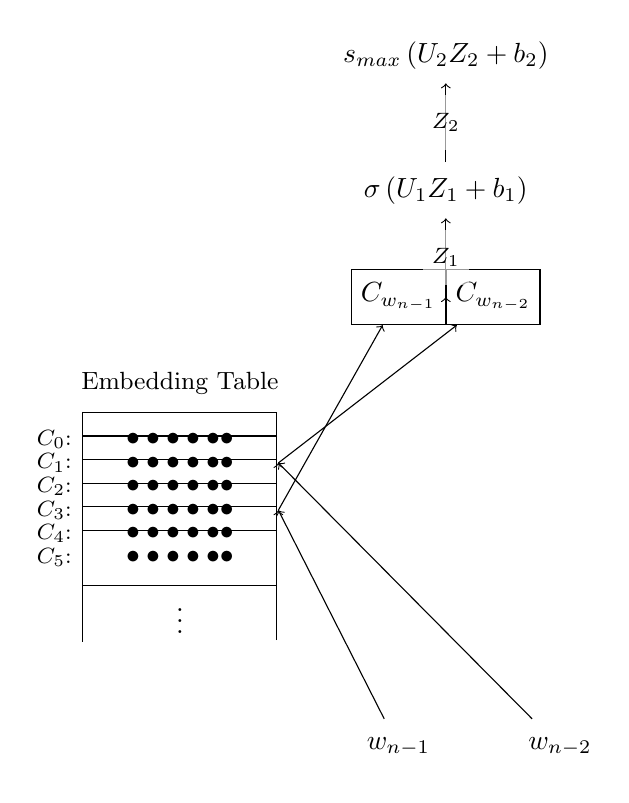
\begin{tikzpicture}[]


\node(w1) {$w_{n-1}$};
\node(w2)[right = of w1] {$w_{n-2}$};


\node(Cn)[lookupbox, above left=of w1] {$\vdots$};
\def\tblmax{6}
\foreach \ii in {1,...,\tblmax} {
	\pgfmathsetmacro\pos{(\ii - 1) * 3 };
	\pgfmathtruncatemacro\jj{(\tblmax -\ii)};
	
	\node(C\ii)[lookupbox, above = \pos mm of Cn]{$\bullet\bullet\bullet\bullet\bullet\bullet$};
	\node(Clbl\ii)[left = 0mm of C\ii]{\footnotesize $C_\jj$:};
};
\node(C)[above = 0mm of C\tblmax] {\small Embedding Table};



\node(concat1)[layer, above = 5 of w1]{$C_{w_{n-1}}$};
\node(concat2)[layer, right = 0 of concat1]{$C_{w_{n-2}}$};

\draw[->] (w1) edge (C3.east);
\draw[->]  (C3.east) edge (concat1);
\draw[->] (w2) edge (C5.east);
\draw[->]  (C5.east) edge (concat2);

\node(L1)[above = of concat1.east]{$\sigma\left(U_1Z_1 + b_1\right)$};
\draw[->]  (concat1.east) edge node[labe]{$Z_1$} (L1);

\node(L2)[above = of L1]{$s_{max}\left(U_2 Z_2 + b_2\right)$};
\draw[->]  (L1) edge node[labe]{$Z_2$} (L2);

\end{tikzpicture}

\end{document} 
	\caption{\label{fig:trigram-neural-language-model} Neural Trigram Language Model}
\end{figure}

In the neural trigram language model, each of the previous two words is used to look-up a vector from the Embedding Table matrix.
These are then concatenated to give a dense, continuous-space input to the above hidden layer.
The output layer is a softmax layer, it gives the probabilities for each word in the vocabulary, one of which corresponds to $w_i$ the word being evaluated.

The word embeddings are trained, via the normal neural network method, along with the network weights and biases.
This allows the embeddings of words which predict the same future word to move to be near each other in vector space.
It also allows the hidden layer to learn to associate information with regions of the embedding space.
This thus allows for information sharing between words.
If two words vectors are close together because they mostly predict the same future words, then that area of space is a associated with predicting those words.
Thus for cases where there are some words which never co-occur in the training set, but for which the nearby word does co-occur with, then because the knowledge is associated with that region of space, the model predicts that there is a higher-than-zero chance of the first word co-occurring with the unseen word.
This is a fuzzy and nonlinear relationship, with varying degrees of closeness resulting in (and from) varying levels of exception of the words sharing co-occurring predicted words.

\subsubsection{Simplified Model considered with input and output embeddings}
When introducing embeddings we considered that one-hot inputs multiplied by matrices
are effectively doing column-lookups which we call embeddings.
Similar same can be said for output layers,
by considering each the output of softmax element-wise it can be reformulated as
\begin{figure}
	\centering
	\caption{\label{fig:trigram-adv-neural-language-model} Neural Trigram Language Model as considered with output embeddings. This is mathematically identical to \Cref{fig:trigram-neural-language-model}}
	\documentclass{standalone}

\usepackage{tikz}
\usetikzlibrary{positioning, fit,  shapes.geometric}
\usepackage{ifthen}
\usepackage{etoolbox}

\tikzset{
	backgroundcolor/.style ={fill=white},
	every node/.append style={
		minimum height=7mm,
	},
	labe/.append style={
		%Blue,
		align = center,
		backgroundcolor,
		fill opacity=0.6,
		text opacity=1,
		font={\footnotesize\itshape}	
	},
	layer/.append style={
		draw,
		align = center,
		minimum height=7mm,
	},
	tight/.append style={
		inner sep=0.2mm,
	},
	lookupbox/.append style={
		draw=none,
		append after command={
		       	[shorten <= -0.5\pgflinewidth]
		       	([shift={(-1.5\pgflinewidth,-0.5\pgflinewidth)}]\tikzlastnode.north east)
		       	edge([shift={( 0.5\pgflinewidth,-0.5\pgflinewidth)}]\tikzlastnode.north west) 
		       	([shift={( 0.5\pgflinewidth,-0.5\pgflinewidth)}]\tikzlastnode.north west)
		       	edge([shift={( 0.5\pgflinewidth,-1.5\pgflinewidth)}]\tikzlastnode.south west)            
		       	([shift={( -1.5\pgflinewidth,+0.5\pgflinewidth)}]\tikzlastnode.south east)
		       	edge([shift={(-1.5\pgflinewidth,-0.5\pgflinewidth)}]\tikzlastnode.north east)
		},
		inner sep=0.7mm,
		outer sep=0mm,
		minimum width=25mm
	}
}
\usepackage{amsmath, amssymb, stmaryrd, mathtools}
\DeclareMathOperator*{\argmin}{argmin}
\DeclareMathOperator*{\argmax}{argmax}

\usepackage{xparse,xstring,etoolbox}
% crossref this against notation section
\newcommand{\vv}[1]{\tilde{#1}} % vector
\newcommand{\seq}[1]{\mathcal{#1}} % sequence
\newcommand{\set}[1]{\mathbb{#1}} % set

%%%%%%%%%
% Indexing/sequence indexing
\newcommand{\seqind}[2]{#1^{#2}} % seqence index
\newcommand{\ind}[2]{#1_{#2}} % indexed
\newcommand{\disamb}[2]{#1^{\mathrm{#2}}} %disambiguated

%% Smart indexing and naming
\newcommand{\ifupper}[3]{
    \normalexpandarg
	\exploregroups
	\StrCount{ABCDEFGHIJKLMNOPQRSTUVWXYZ}{#1}[\uppercount]
	\ifnumgreater{\uppercount}{0}{#2}{#3}
}

%smart index
\DeclareDocumentCommand{\ii}{u{_} m}{
	\ifupper{#1}%
	{% just a single uppercase character, i.e. a matrix
		  %make sure the index is the right length
		\StrCount{#2}{,}[\indcount]
		\ifnumgreater{\indcount}{0}
		{ % Got multiple indexes so all good
		 	\ind{#1}{#2}
		}
		{ % Only 1 index so grab the column
		 	\ind{#1}{{:,#2}}
		}
	}%
	{% Not just a single upper case character
		\ind{#1}{#2}
	}
}

\DeclareDocumentCommand{\nn}{u{_} m}{
	\seqind{#1}{#2}
}

\DeclareDocumentCommand{\dd}{u{_} m}{
	\disamb{#1}{#2}
}

% Index of a vector
\DeclareDocumentCommand{\iv}{u{_} m}{\ii{\vv #1}_{#2}}
\DeclareDocumentCommand{\dv}{u{_} m}{\dd{\vv #1}_{#2}}
\DeclareDocumentCommand{\nv}{u{_} m}{\nn{\vv #1}_{#2}}

%exp
\let\oldexp\exp
\renewcommand{\exp}[1]{\oldexp \left( #1 \right)}
\newcommand{\exptwo}[1]{\oldexp_2 \left( #1 \right)}

\newcommand{\softmax}{\mathrm{smax}}

\DeclareMathOperator*{\expectedop}{\mathbb{E}}
\DeclareDocumentCommand{\expected}{u{_} m}{
	\expectedop\limits_{\mathrlap{#2}}
}
\usetikzlibrary{calc}
\begin{document}

\begin{tikzpicture}[]


\node(w1) {$\n w_{i-1}$};
\node(w2)[right = of w1] {$\n w_{i-2}$};


\node(Cn)[lookupbox, above left=of w1] {$\vdots$};
\def\tblmax{6}
\foreach \ii in {1,...,\tblmax} {
	\pgfmathsetmacro\pos{(\ii - 1) * 3 };
	\pgfmathtruncatemacro\jj{(\tblmax -\ii)};
	
	\node(C\ii)[lookupbox, above = \pos mm of Cn]{$\bullet\bullet\bullet\bullet\bullet\bullet$};
	\node(Clbl\ii)[left = 0mm of C\ii]{\footnotesize $\i C_\jj$:};
};
\node(C)[above = 0mm of C\tblmax.north, text width=40] {\small \textsc{Input \\Embedding Table}};


\node(concat1)[layer, above = 5 of w1]{$\i C_{\n w_{i-1}}$};
\node(concat2)[layer, right = 0 of concat1]{$\i C_{\n w_{i-2}}$};

\draw[->] (w1) edge (C3.east);
\draw[->]  (C3.east) edge (concat1.south);
\draw[->] (w2) edge (C5.east);
\draw[->]  (C5.east) edge (concat2.south);

\node(L1)[layer, above = of concat1.north east]{$\varphi\left(U\,\dv z_{embs} + \v b\right)$};
\draw[->]  (concat1.north east) -- node[labe]{$\dv z_{embs}$} (L1);

$\frac{\exp{\i V_{\n w_i,:} \dv z_{hid} + \iv k_{\n w_i,:}}}%
{\sum_{\forall j} \exp{\i V_{j,:} \dv z_{hid} + \iv k_j}}$
};
\draw[->]  (L1) edge node[labe]{$\dv z_{hid}$} (L2);


\node(out)[above = of L2]{$P(\n w_i \mid \n w_{i-1}, \n w_{i-2})$};
\draw[->] (L2) edge (out);

\node(Vn)[lookupbox, above = 5 of Cn] {$\vdots$};
\def\tblmax{6}
\foreach \ii in {1,...,\tblmax} {
	\pgfmathsetmacro\pos{(\ii - 1) * 3 };
	\pgfmathtruncatemacro\jj{(\tblmax -\ii)};
	
	\node(V\ii)[lookupbox, above = \pos mm of Vn]{$\bullet\bullet\bullet\bullet\bullet\bullet$};
	\node(Vlbl\ii)[left = 0mm of V\ii]{\footnotesize $\i V_{\jj,:}$:};
	
	\pgfmathsetmacro\ang{(\ii * -2 + -180+20 };
	\draw[->] (V\ii.east) -- (L2.\ang);
};
\draw[->] (Vn.east) -- (L2.south west);
\node(C)[above = 0mm of V\tblmax.north, text width=40] {\small \textsc{Output \\Embedding Table}};




\draw[->] (out.204) -- (V6.east);
\draw[->] (V6.east)-- (L2.120);

\end{tikzpicture}

\end{document} 
\end{figure}


With the final layer being defined as:
\begin{equation}
s_{max}(Vz_{2}+k) = \dfrac{\exp\left(V_{w_{i}}^{T}z_{2}+k_{i}\right)_{i=0}^{i=N}}{\sum_{\forall j}exp\left(V_{j}^{T}z_{2}+k_{j}\right)}
\end{equation} 

In this formulation, we have $V_{w_{i}}^{T}$ as the output embedding
for $w_{i}$ -- an output word.
As we considered  $C_{w_{i}}$ as its input embedding.

Further, $V_{w_{i}}^{T}z_{2}$ can be seen as computing the dot product
between the output embedding for $w_{i}$ and the hidden layer representation
of $w_{i-1}$ and $w_{i-2}$ in the form of $z_{2}$. 

It is also clear when we look at the Bayes-like reformulation: (See \Cref{sec:softmax-and-bayes-theorem})
\begin{equation}
P(Y=y\mid Z=z)=\frac{R(Z=z\mid Y=y)\,Q(Y=y)}{\sum_{\forall i}R(X=x\mid Y=i)\,Q(Y=i)}
\end{equation}

Which in this case is:
\begin{equation}
P(w_{i}\mid w_{i-1},w_{i-2})=\frac{R(Z=z_{2}\mid W_{i}=w_{i})\,Q(W_{i}=w_{i})}{\sum_{\forall j}R(Z=z_{2}\mid W_{i}=w_{j})\,Q(W_{i}=w_{j})}
\end{equation}

where $Q(Y=y)=e^{k}$ -- this is linked to the Unigram word probabilities. $P(Y=y)$
Such that one might suggest a good value for $k$ to be given by the log unigram probabilities: $k=\left(\log P(W_{i}=w_{j})\right)_{j=1}^{j=N}$.
If $\mathbb{E}(R(Z\mid W_{i})=1$ then this would be optimal.
That condition is equivalent to if $\mathbb{E}(VZ_{2})=0$
Given the $V$ is normally initialized as a zero mean Gaussian, this condition is at least initially true.

\subsubsection{The Neural Probabilistic Language Model}
\tcite{NPLM} is a more advanced version of the neural language model discussed.
Rather than being a trigram language model, it is an $n$-gram language model, where $n$ is a hyper-parameter of the model.
The knowledge sharing allows the data-sparsity issues to be ameliorated, thus allowing for $n>3$.
%
\aside{\textcite{schwenk2004efficient} suggests using only a subset of the vocabulary as options for the output, while allowing the full vocabulary in the input space -- with a fallback to classical language models for the missed words.
	This decreases the size of the softmax output layer, substantially decreasing the network evaluation and training time.
	This technique is now largely eclipsed by hierarchical softmax etc. discussed later in this chapter.
}
%
Bengio et. al. investigates values for $n$ of 3, 5 and 6.
The network used in their work also was marginally more complex, as shown in \Cref{fig:neural-language-model} and in the following equation:
\begin{align}
P(w_i & \mid w_{i-1}, w_{i-2}) = s_{max}( \nonumber
\\  & \quad U_3 \left[ C_{w_{i-1}};...; C_{w_{i-n}}\right] \nonumber
\\  & + V \: \varphi\left( U\left[C_{w_{i-1}};...; C_{w_{i-n}} \right] + b_1\right) \nonumber
\\  & +b_2)
\end{align}

It includes a layer-bypass, which is primarily present only as connivance to aid in the learning.
It allowing the input to directly effect the output without being mediated by the shared hidden layer.
This layer-bypass is a unusual feature, not present in future works deriving from this, such as \tcite{schwenk2004efficient} which presents a bag of tricks to minimize training time. 


This is the network which begins the notions of using neural networks with vector representations of words.
Bengio et. al. focused on the use of the of sliding window of previous words -- much like the traditional n-grams.
At each time-step the window is advanced forward and the next word predicted based on that shifted context of prior words.
They do very briefly mention that an RNN could be used in its place.

\begin{figure}
	\centering
	\documentclass{article}

\usepackage{tikz}
\usetikzlibrary{positioning, fit,  shapes.geometric}
\usepackage{ifthen}
\usepackage{etoolbox}

\tikzset{
	backgroundcolor/.style ={fill=white},
	every node/.append style={
		minimum height=7mm,
	},
	labe/.append style={
		%Blue,
		align = center,
		backgroundcolor,
		fill opacity=0.6,
		text opacity=1,
		font={\footnotesize\itshape}	
	},
	layer/.append style={
		draw,
		align = center,
		minimum height=7mm,
	},
	tight/.append style={
		inner sep=0.2mm,
	},
	lookupbox/.append style={
		draw=none,
		append after command={
		       	[shorten <= -0.5\pgflinewidth]
		       	([shift={(-1.5\pgflinewidth,-0.5\pgflinewidth)}]\tikzlastnode.north east)
		       	edge([shift={( 0.5\pgflinewidth,-0.5\pgflinewidth)}]\tikzlastnode.north west) 
		       	([shift={( 0.5\pgflinewidth,-0.5\pgflinewidth)}]\tikzlastnode.north west)
		       	edge([shift={( 0.5\pgflinewidth,-1.5\pgflinewidth)}]\tikzlastnode.south west)            
		       	([shift={( -1.5\pgflinewidth,+0.5\pgflinewidth)}]\tikzlastnode.south east)
		       	edge([shift={(-1.5\pgflinewidth,-0.5\pgflinewidth)}]\tikzlastnode.north east)
		},
		inner sep=0.7mm,
		outer sep=0mm,
		minimum width=25mm
	}
}

\begin{document}

\begin{tikzpicture}[]


\node(w1) {$\n w_{i-1}$};
\node(w2)[right = 0mm  of w1] {$\n w_{i-2}$};
\node(w3)[right = 0mm of w2] {$\ldots$};
\node(w4)[right = 0mm of w3] {$\n w_{i-n}$};


\node(Cn)[lookupbox, above left=of w1] {$\vdots$};
\def\tblmax{6}
\foreach \ii in {1,...,\tblmax} {
	\pgfmathsetmacro\pos{(\ii - 1) * 3 };
	\pgfmathtruncatemacro\jj{(\tblmax -\ii)};
	
	\node(C\ii)[lookupbox, above = \pos mm of Cn]{$\bullet\bullet\bullet\bullet\bullet\bullet$};
	\node(Clbl\ii)[left = 0mm of C\ii]{\footnotesize $\i C_\jj$:};
};
\node(C)[above = 0mm of C\tblmax] {\small \textsc{Embedding Table}};


\node(concat1)[layer, above = 5 of w1]{$\i C_{\n w_{i-1}}$};
\node(concat2)[layer, right = 0 of concat1]{$\i C_{\n w_{i-2}}$};
\node(concat3)[layer, right = 0 of concat2]{$\quad\ldots\quad$};
\node(concat4)[layer, right = 0 of concat3]{$\i C_{\n w_{i-n}}$};
 
\draw[->] (w1) edge (C3.east);
\draw[->]  (C3.east) edge (concat1.south);
\draw[->] (w2) edge (C5.east);
\draw[->]  (C5.east) edge (concat2.south);
\draw[->] (w4) edge (C5.east);
\draw[->]  (C5.east) edge (concat4.south);

\node(L1)[layer, above = of concat2.north east]{$\varphi\left(\d U_{hid}\dv z_{embs} + \v b\right)$};
\draw[->]  (concat2.north east) -- node[labe]{$\dv z_{embs}$} (L1);


\node(L2)[layer, above = of L1]{$s_{max}\left(V \dv z_{hid} +\d U_{bypass} \dv z_{embs}+ \v k\right)$};
\draw[->]  (L1) edge node[labe]{$\dv z_{hid}$} (L2); 
\draw[->, bend right] (concat2.north east)  to[bend right=45, min distance=25 mm] (L2);


\node(out)[above = of L2]{$P(\n w_i \mid \n w_{i-1}, \n w_{i-2}, \ldots, \n w_{i-n})$};
\draw[->] (L2) edge (out);


\end{tikzpicture}

\end{document} 
	\caption{\label{fig:neural-language-model} Neural Probabilistic Language Model}
\end{figure}


\subsection{RNN Language Models}

\pdfcomment{I'm not sure if Mikolov was using the design matrix formulatiuon where bias terms are skipped, if so this section is the only section so far that skips it}

\aside[Differences in formulation]{
The network and equations shown here may seem different to those presented in \textcite{mikolov2010recurrent}.
However they are mathematically identical.
The apparent difference is simply the choice between considering embeddings as a look-up, or as a one-hot multiplication.
}

In \tcite{mikolov2010recurrent} an RNN is for a language model.
To be precise, an Elman network is used \tcite{elman1990finding}.
In this form of RNN, the output of hidden layer in the previous time-step is appended as an additional input.
Using an RNN eliminates the sliding window of earlier language models.
Instead, the context information is stored in the state that is passed forward.

This state $Z_{j}$ being the hidden state output from the first (only) hidden layer when input the $j$th word, 
is given by 

\begin{equation}
	Z_{j} = \varphi\left( U\,Z_{j-1} + C_{w_{i-1}} \right)
\end{equation}


This hidden layer was the an input to the hidden-layer at the next time-step, as well as to the output softmax.

\begin{equation}
	P(w_i \mid w_{i-1}, ... w_{1}) = s_{max}\left(V \, Z_{i-1} \right)
\end{equation}



Rather than using an Elman network, a more advanced RNN such as Long-Short-Term-Memory (LSTM), or a Gated Recurrent Unit (GRU) \pcite{cho2014properties}, based network could be used.
The structure would remain very similar,
and additional advantages may be found from the improved stability and performance.

\tcite{sundermeyer2012lstm} investigated using LSTM.
This did indeed offer an improvement over the Elman network used in \textcite{mikolov2010recurrent}.
\tcite{jozefowicz2015empirical} conducted an extensive search of hyper-parameters for LSTM and GRU networks for language modeling.
For the best performing networks of both types the results found were significantly better than \textcite{sundermeyer2012lstm} and \textcite{mikolov2010recurrent}.
They found the best was the LSTM network, particularly if the forget gate was biased to a 1.0 or more.

\begin{figure}
	\centering
	\documentclass{article}

\usepackage{tikz}
\usetikzlibrary{positioning, fit,  shapes.geometric}
\usepackage{ifthen}
\usepackage{etoolbox}

\tikzset{
	backgroundcolor/.style ={fill=white},
	every node/.append style={
		minimum height=7mm,
	},
	labe/.append style={
		%Blue,
		align = center,
		backgroundcolor,
		fill opacity=0.6,
		text opacity=1,
		font={\footnotesize\itshape}	
	},
	layer/.append style={
		draw,
		align = center,
		minimum height=7mm,
	},
	tight/.append style={
		inner sep=0.2mm,
	},
	lookupbox/.append style={
		draw=none,
		append after command={
		       	[shorten <= -0.5\pgflinewidth]
		       	([shift={(-1.5\pgflinewidth,-0.5\pgflinewidth)}]\tikzlastnode.north east)
		       	edge([shift={( 0.5\pgflinewidth,-0.5\pgflinewidth)}]\tikzlastnode.north west) 
		       	([shift={( 0.5\pgflinewidth,-0.5\pgflinewidth)}]\tikzlastnode.north west)
		       	edge([shift={( 0.5\pgflinewidth,-1.5\pgflinewidth)}]\tikzlastnode.south west)            
		       	([shift={( -1.5\pgflinewidth,+0.5\pgflinewidth)}]\tikzlastnode.south east)
		       	edge([shift={(-1.5\pgflinewidth,-0.5\pgflinewidth)}]\tikzlastnode.north east)
		},
		inner sep=0.7mm,
		outer sep=0mm,
		minimum width=25mm
	}
}

\begin{document}

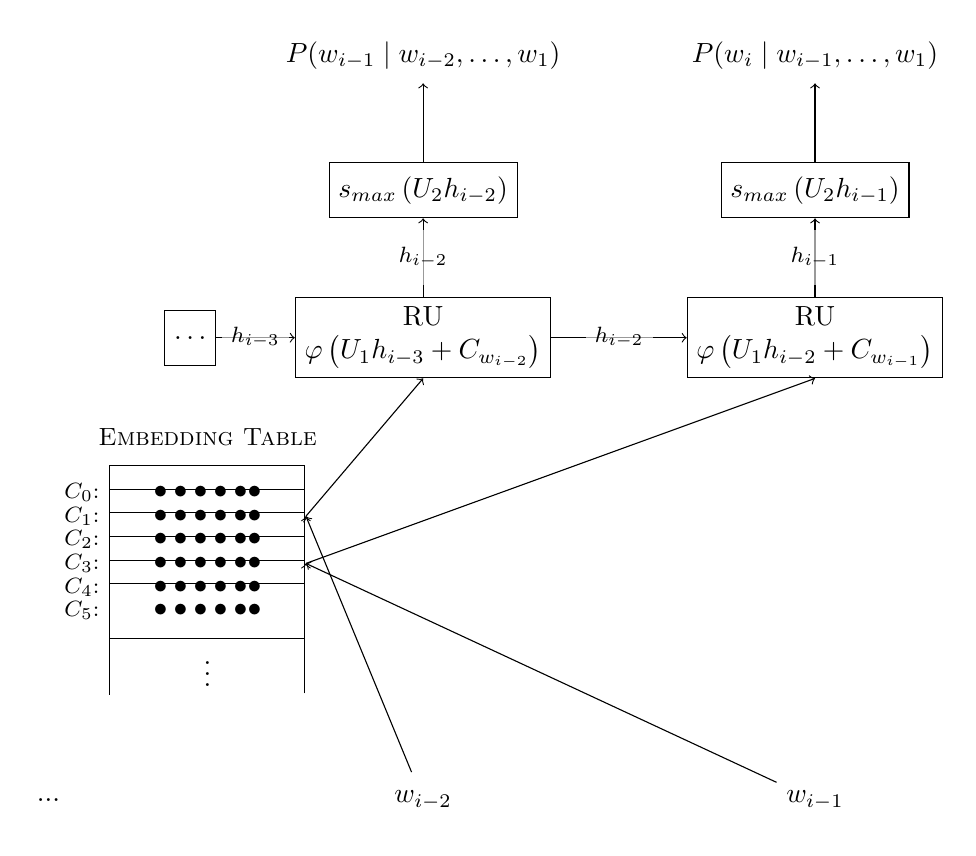
\begin{tikzpicture}[]

\newcommand{\hsep}{4}
\newcommand{\vtablesep}{5}

\node(w1) {$w_{i-1}$};
\node(w2)[left = \hsep of w1] {$w_{i-2}$};
\node(w3)[left = \hsep of w2] {$...$};


\node(Cn)[lookupbox, above left=of w2] {$\vdots$};
\def\tblmax{6}
\foreach \ii in {1,...,\tblmax} {
	\pgfmathsetmacro\pos{(\ii - 1) * 3 };
	\pgfmathtruncatemacro\jj{(\tblmax -\ii)};
	
	\node(C\ii)[lookupbox, above = \pos mm of Cn]{$\bullet\bullet\bullet\bullet\bullet\bullet$};
	\node(Clbl\ii)[left = 0mm of C\ii]{\footnotesize $C_\jj$:};
};
\node(C)[above = 0mm of C\tblmax] {\small \textsc{Embedding Table}};

\node(L11)[layer, above = \vtablesep of w1]{RU\\$\varphi\left( U_1h_{i-2}  +  C_{w_{i-1}}\right)$};
\node(L21)[layer, above = of L11]{$s_{max}\left(U_2 h_{i-1}\right)$};
\draw[->]  (L11) edge node[labe]{$h_{i-1}$} (L21);
\node(out1)[above = of L21]{$P(w_i \mid w_{i-1}, \ldots,  w_1)$};
\draw[->] (L21) edge (out1);

\node(L12)[layer, above = \vtablesep of w2]{RU\\$\varphi\left( U_1h_{i-3}  +  C_{w_{i-2}}\right)$};
\node(L22)[layer, above = of L12]{$s_{max}\left(U_2 h_{i-2} \right)$};
\draw[->]  (L12) edge node[labe]{$h_{i-2}$} (L22);
\node(out2)[above = of L22]{$P(w_{i-1} \mid w_{i-2}, \ldots,  w_1)$};
\draw[->] (L22) edge (out2);
\draw[->]  (L12) edge node[labe]{$h_{i-2}$} (L11);

\node(L13)[layer, left = of L12] {$\ldots$};
\draw[->]  (L13) edge node[labe]{$h_{i-3}$} (L12);


\draw[->] (w1) edge (C3.east);
\draw[->]  (C3.east) edge (L11.south);
\draw[->] (w2) edge (C5.east);
\draw[->]  (C5.east) edge (L12.south);


\end{tikzpicture}

\end{document} 
	\caption{\label{fig:neural-language-model} RNN Language Model}
\end{figure}

This ends our discussion of standard language models.


\section{Acausal Language Modeling}
The step beyond a normal language model,
which uses the prior words to predict the next word,
is what we will term acausal language modelling.
Here we use the word acausal in the signal processing sense.
The task here is to predict a missing word, using the words the preceed it, as well as the words that come after it.

As it is acausal it can not be done in a real-time system, and is not useful for many tasks directly.
However, what it is very useful for is as a task to learn a good representation for words.


\subsection{Context RNN}


\aside[Are CBOW \& Skip-Gram Neural Networks]{As these models do not have any non-linearities  (some would say they have no hidden layer, though is is incorrect: the projection layer of the embedding is functionally a hidden layer) it may be asserted that they are not in-fact neural networks at all.
This distinction is purely academic though.
Any toolkit that can well handle the prior discussed neural network models, can be very well used to implement CBOW and Skip-Gram.
}


\pdfcomment{I think CBOW and Skip-Gram don't feature Biases because they are written in Design Matrix form with a column of ones. If so I need to fix that up to something consistent with the remainder of this chapter or if not then }

These works, which introduced the CBOW and Skip-Gram is also responsible for the popularisation of Hierarchical Softmax and Negative Sampling methods.
As these are complicated and often misunderstood, topics in their own right, they are discussed in a more tutorial fashion in \Cref{sec:hierachical-softmax-and-negative-sampling} 

\subsection{CBOW}\label{sec:cbow}
The continuous bag of words (CBOW) method was introduced by \tcite{mikolov2013efficient}.
In truth this is not particularly similar to bag of words at all, no more so than any other word representation that does not have regard for order of the context words (e.g. skip-gram, GloVE below).


For a context window of width $n$ words -- i.e. $\frac{n}{2}$ words to either side, of the target word,
the CBOW model is defined by:
\begin{align}
P(w_i & \mid w_{i-\frac{n}{2}},..., w_{i-1}, w_{i+1},...,w_{i+\frac{n}{2}})  \nonumber
\\  & = s_{max}(U \sum_{j=i+1}^{j=\frac{n}{2}} \left( C_{w_{i-j}}+C_{w_{i+j}} \right))
\end{align}

\pdfcomment{Need to consider that this is always done with a Hierarchical softmax, and check this formulation is correct}



\subsection{Skip-gram}\label{sec:skip-gram}
\aside[Skip-gram naming]{In different publications this model may be called skipgram skip-gram, skip-ngram, skip-gram etc. Further, it may be called \texttt{word2vec} after the publicly released implementation of the algorithm. Though that software also can be used for CBOW.}


The converse of CBOW is the skip-grams model \tcite{mikolov2013efficient}.
In this model, the central word is used to predict the words in the context.
While in CBOW each training case of context and target word presents one correct answer,
in the Skip-gram each training case has a number of correct answers, the probability of all of which in the softmax must be increased.

\begin{equation}
P(w_j \mid w_{i}) = \left[ s_{max}(V\,C_{w_{i}}) \right]_{w_j} 
\end{equation}


The goal, is to maximise the probabilities of all the observed outputs from the window's in the training set ($i-\frac{n}{2},...,i-1, i+i,...,i+\frac{n}{2}$).
This can be done using softmax, or hierarchical softmax, or an approximation call negative sampling
(Hierarchical softmax and negative sampling are discussed in \Cref{sec:hierachical-softmax-and-negative-sampling}).
It should be understood that while this is presented similarly to a classification task,
there is no expectation that the model will actually predict the correct result,
given that there is even during training multiple correct results -- every word from the window.


Note that Skip-Grams only hidden layer is the embedding layer.
If we take the earlier discussed notion of considering the output matrix $V$ as being an embedding layer
then this becomes:

\begin{align}
P(w_j \mid w_{i}) & = \left[ s_{max}(V\,C_{w_{i}}) \right]_{w_j} \\
P(w_j \mid w_{i}) & = \frac{\exp(V_{w_j}^\prime\,C_{w_{i}})}{\sum_{k=1}^{k=N} \exp(V_k^\prime\,C_{k})}
\end{align}

The key term here is the $V_{w_j}^\prime\,C_{w_{i}}$,
the remainder of the expression is normalising this into a probability.
Maximising the probability $P(w_j \mid w_{i})$ is equivalent to maximising the dot produce between $V_{w_j}^\prime$, the output embedding for $w_j$ and  $C_{w_i}$ the input embedding for $w_i$.
Which is to say that the skip-gram probability is maximises when the angular difference between the input embedding for a word, and the output embeddings for words that it co-occurs with is minimised, and the embeddings themselves are maximised.
\pdfcomment{Does maximising the embedding cancel out?}.


While skip-gram and CBOW were introduces in the same set of papers, subsequent work has found the skip-gram is almost always the preferred system for any task. \pdfcomment{Citation for this?}

\subsection{Analogy Tasks}
\aside[Analogy Tasks uncover prejudice in corpora]{\textcite{bolukbasi2016man} and \textcite{Caliskan183} use analogy tasks, and related variant formulations to find troubling associations between words, such as Bolukbasi et. al's titular \natlang{Man} is to \natlang{Computer Programmer}, as \natlang{Woman} is to \natlang{Homemaker}. Finding these relationships in the embedding space, indicated that they are present in the training corpus, which in turn shows their prevalence  in society at large.
As has been observed: Machine learning can be a very good mirror.
}



\asidefig[\label{fig:analogy}Example of analogy algebra]{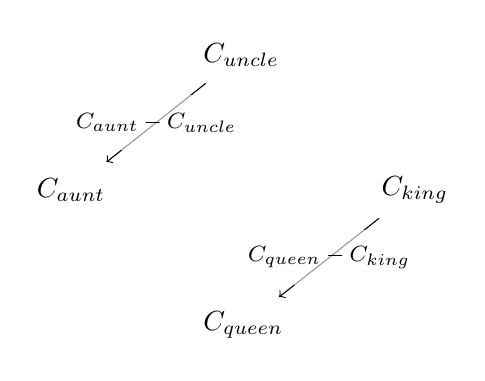
\begin{tikzpicture}
\node(a) {$C_{aunt}$};
\node(b)[above right = of a] {$C_{uncle}$};
\node(c)[below right = of a] {$C_{queen}$};
\node(d)[above right = of c] {$C_{king}$};

\draw[->] (b) -- (a) node[labe,midway]{$C_{aunt}-C_{uncle}$};
\draw[->] (d) -- (c) node[labe,midway]{$C_{queen}-C_{king}$};
\end{tikzpicture}
}

\asidefig[\label{fig:anavecs} Vectors involved in analogy ranking tasks, this may help to understand the math]{
	\begin{tikzpicture}
	\node(a) {$C_a$};
	\node(b)[above right = of a] {$C_b$};
	\node(c)[below right = of a] {$C_c$};
	\node(d)[above right = of c] {$C_d$};
	
	\draw[->] (b) -- (a) node[labe,midway]{$C_a-C_b$};
	\draw[->] (d) -- (c) node[labe,midway]{$C_d-C_c$};
	\end{tikzpicture}
}

It is on these systems that evaluation the analogy tasks became well known, though they were considered earlier on RNN neural language models \pcite{mikolov2013linguisticsubstructures}.
These tasks are keyed around answering the question: What is  \emph{c} and \emph{b} is to \emph{a}.
For example, a semantic analogy would be answering that \natlang{Aunt} is to \natlang{Uncle} as \natlang{King} is to \natlang{Queen}.
For example, a syntactic analogy would be answering that \natlang{Kings} is to \natlang{King} as \natlang{Queens} is to \natlang{Queen}.
The latest and largest analogy test set is presented by \tcite{gladkova2016analogy},
which evaluates embedding on 40 subcategories of knowledge.




The analogies work by relating similarities of offsets.
\pdfcomment{fix this to refer to analogy figure}
Word similarity can be evaluated using word embeddings using a number of metrics.
By far the cosine similarity is the most common.
This is given by 

\begin{equation}
sim(C_u, C_v)=\frac{C_{u}\cdot C_{v}}{\left\Vert u\right\Vert \left\Vert v\right\Vert }
\end{equation}
A smaller distance in vector space, means the words are more similar -- in some sense.
Depending on the system this similarity could be syntactic, semantic or otherwise, the analogy tasks can help identify what kinds of similarities the embeddings are capturing.

Using the similarity scores a ranking of words to complete the analogy is found.
To find the correct word for \emph{d} in: \emph{d} is to \emph{c} as \emph{b} is to \emph{a}
the following is computed for the table of embeddings $C$:
\begin{align}
\qquad & \argmax_{\forall d} sim(C_d - C_c, C_a-C_b)\\
\text{i.e} & \argmax_{\forall d} sim(C_d, C_a-C_b+C_c)
\end{align}

%The motivational diagram is shown in \Cref{fig:anavecs}
\pdfcomment{insert reference to figure here}


Initial results were relatively poor, but the surprising finding was that this worked at all \cite{mikolov2013linguisticsubstructures}.
Subsequent results found in \tcite{pennington2014glove} and other works were significantly better than the initial results.

\section{Co-location Factorisation}

\subsection{GloVe}

Skip-grams are intrinsically prediction based methods, effectively predicting what words will co-occur in the context of a local window and optimising as such.
In \tcite{pennington2014glove}the authors show that if one were to change that optimisation to be global over all co-occurrences,
then the optimisation critia becomes minimising the cross-entropy between the true co-occurrence probabilities given by $P(w_j\mid w_j)$, and the value of the embedding product: the cross entropy measure.,
weighted by the frequency of the occurrence of the word $X_i$.
That is to say if skip-gram were optimised globally it would be equivalent to minimising:
\begin{equation}
J = - \sum_{\forall w_i} \sum_{\forall w_j} X_{ij} P(w_j\mid w_j) \log (V_{w_j}^\prime\,C_{w_{i}})
\end{equation}

Minimising this cross-entropy efficiently means factorising the true co-occurrence matrix,
into the input and output embedding matrices $C$ and $V$, under a particular set of weightings given by the cross entropy measure.

\tcite{pennington2014glove} consider instead factorizing the logarithm of co-occurrence matrix directly,
the logarithm giving an different, but similar, weighting to the cross entropy measure.
Thas is for each word co-occurrence of $w_i$ and $w_j$: Attempting to find optimal values for 
the embeddings $C_{w_{i}}$, and $V_{w_j}^\prime$, while also allowing constant offsets $b_i$ and $k_j$
such that:
$V_{w_j}^\prime\,C_{w_{i}} + b_i + k_j \approx \log(X_{ij})$
as near as is possible.

\aside[Implementing GloVe]{To implement GloVe in any technical programming language with good support for matrix factorisation via least-squares optimisation is trivial. As is implementing any other matrix factorisation/dimensionality reduction based method.}

The precise measure used to do this, is a weighted the least squares minimisation of 
\begin{equation}
J = - \sum_{\forall w_i}  \sum_{\forall w_j} f(X_{ij})\,V_{w_j}^\prime\,C_{w_{i}}+b_i+k_j-\log (X_ij)
\end{equation}


using the weighting between 0 and 1 given by $f(x)$
\begin{equation}
f(x)=\begin{cases}
\left(\frac{x}{100}\right)^{0.75} & x<100\\
1 & otherwise
\end{cases}
\end{equation}
though they suggest other weightings may be suitable.
This can be contrasted as a saturating variant of the effective weighing of skip-gram being $X_{ij}$.
Though the variation in measure away from cross-entropy also significant and has related effects on the weightings of rare vs common words in the minimisation.

While in initial tests it was found that Glove out-performed  skip-gram,
subsequent more extensive testing in \tcite{levy2015lsaisbasicallyskipgramswithexperimentstoprove} with more tuned parameters,
found that skip-gram out-performed GloVE on all tasks, though the performance is relatively comparable.



\aside[Key Factors Mentioned as Minor Tweaks]{
There is an interesting pattern of important factors being considered as not part of the core algorithm.
GloVe explicitly weights all co-occurrences inversely by the distance from each other -- though this is considered part of finding the co-occurrence matrix rather than part of the algorithm itself.
Skip-Gram accomplishes something similar with dynamic window sizing tweak -- the true size of the window is uniformly distributed between 1 and the value given.

GloVe explicitly scales the weight of terms to be optimised -- using the weighting function, which saturates for frequent terms.
Skip-Gram accomplishes something similar again using the sub-sampling tweak -- common words are randomly skipped from the contexts during training, based on how common they are.

While the original papers consider these as unimportant to the main thrust of the algorithms \textcite{levy2015lsaisbasicallyskipgramswithexperimentstoprove} found them to be crucial hyper-parameters.
}

However, GloVe loosely highlights the relationship between the co-located word prediction neural network models,
and the more traditional matrix factorization of collocation counts used in topic modeling.
Very similar properties were also explored for skip-grams with negative sampling in \tcite{levy2014neural} and then in \tcite{li2015wordemedingasEMF} with more direct mathematical equivalence to weighed co-occurrence matrix factorisation;
Later in \tcite{cotterell2017SkipgramisEPCA} showed the equivalence to exponential principal component analysis.
\tcite{wordvecispca} goes on the extend that show that it is a weighted logistic principal component analysis, which is a special case for of the exponential.
There are many works in this area now.


\subsection{Conclusion}
As we have now concluded that neural predictive co-location models are functionally very similar to matrix factorisation of co-location counts with suitable weightings, and suitable similarity metrics.
One might suggest a variety of word embeddings to be created from a variety of different matrix factorisations with different weightings and constraints; and indeed this has been done.
Traditionally large matrix factorisations have significant problems in terms of computational time and memory complexity.
A common solution to this is to handle it an iterative optimisation procedure.
Training a neural network such as skip-gram is an iterative optimisation procedure.




\section{Hierarchical Softmax and Negative Sampling}\label{sec:hierachical-softmax-and-negative-sampling}

\subsection{Hierarchical Softmax}
Hierarchical softmax was first presented in  \tcite{morin2005hierarchical}.
It's recent use was popularised by \tcite{mikolov2013efficient}, where is is used using a huffman tree.



\aside[SemHuff]{It can be noted that the huffman encoding scheme specifies only the depth of a given word in the tree. It does not specify the order.
	\textcite{SemHuff} makes use of the BlossomV algorithm \parencite{Kolmogorov2009} to sort the nodes on each layer according to their similarity.
	They found that on the language modelling task this improved performance, in the way one would expect.
	They used a lexical resource to determine similarity, however noted that one could use a prior trained word2vec model as the similarity measure.
	This is very similar to the original method used by \parencite{morin2005hierarchical},
	but only using the similarity measure for reordering nodes at the same depth, after the depth is decided by huffman encoding.
	This is a fun method to implement and is interesting.
	In our own experimentation with it on other tasks, we were not actually seeing large improvements.
	As a more obscure method it is worth benchmarking for new tasks.
}

One of the most expensive parts of training and using a neural language model is calculating the softmax final layer.
As the softmax denominator includes terms for each word in the vocabulary, the computation of all of them is expensive.
\pdfcomment{write more intro here. Refer to the Output vector formulation}

In hierarchical softmax, each word (output choice), is considered as a leaf on a binary tree.
The tree is normally a Huffman tree \pcite{huffman1952method}, as was found to be effective by \tcite{mikolov2013efficient}.
This which means that for each word $w_i$, the words depth (i.e its code's length) $L(w_i)$ is such that over all words: $\sum_{\forall w_j \in \mathcal{V}} P(w_j)\times L(w_j)$ is minimised.
Where $P(w_i)$ is word $w_i$'s unigram probability, and $\mathcal{V}$ is the vocabulary.
The approximate solution to this is that $L(w_i) \approx -\log_2(P(w_i))$.
From the tree each work is can be assign as code in the usual way, with 0 for example representing taking one branch, and 1 representing the other.
Each point in the code corresponding to a node, which has decision tied to it.
This code is used to transform the large  multinomial softmax classication into a series of binary logistic classifications.
It is important to understand the layers in the tree are not layers of the neural network.
They are in-fact subsets of the neurons on the output layer, with a relationship imparted on them.

As is noted by \tcite{mikolov2013efficient}, for a vocabulary $\mathcal{V}$,
using a normal softmax would require each evaluation to perform $|\mathcal{V}$ operations;
using hierarchical softmax with a balanced tree, would mean the expected number of operations across all words would be $\log_2(|\mathcal{V}|)$;
but using huffman encoding gives expected number of operations $\sum_{\forall w_j \in \mathcal{V}} -P(w_j)\log_2(P(w_i)) = H(\mathcal{V})$, where $H(\mathcal{V})$ is the entropy (in the information theoretic sense) of the unigrams in the vocabulary.
The worse case value for that entropy is $\log_2(|\mathcal{V}|)$.
In-fact huffman encoding is provably optimal in this way, so this is the minimal number of operations required in the average case.


\subsubsection{An incredibly gentle introduction to hierarchical softmax}

In this section for brevity we will ignore the bias component of each decision at each node.
It can either be handled nearly identically to the weight;
or the matrix can be tank in \emph{design matrix form} with an implicitly appended column of ones;
or it can actually be ignored in implementation.
The reasoning for ignoring it in implementation is that the normal softmax bias encodes unigram probabilities;
in Hierarchical softmax when used with the common Huffman encoding its depth in tree encodes its unigram probability. In this case, not using bias would at most cause error proportionate to $2^{-k}$, where $k$ is the smallest integer such that $2^{-k}>P(w_i)$.
\pdfcomment{this seems right, but idk if it is. I need to check this}

% settings for trees
\tikzset{every internal node/.style={draw, circle, tight}}

\paragraph{First consider a binary tree with just 1 layer and 2 leaves}
The leaves are $n_{00}$ and $n_{01}$, these leaf notes each correspond to a word from the vocabulary.


\aside{\begin{tikzpicture}
	\Tree [.$n_0$ 
		$n_{00}$
		$n_{01}$ ]
\end{tikzpicture} Tree for 2 words}
	
We are at the initial root which we call $n_{0}$, and we can go to
either node $n_{00}$ or node $n_{01}$, based on the input from the
layer below which we will call $z$.

Here we write $n_{01}$ to represent the event of the first nonroot
node being the branch given by following the 0th branch, vs the $n_{01}$
being to follow the first branch. 

We are naming the root node as a notation convenience so we can talk
about the decision made at $n_{0}$. note that $P(n_{0})=1$.

We want to know the probability of the next node being the 0th (i.e.
$P(n_{00}\mid z)$ ) or the first (i.e. $P(n_{01}\mid z)$).

We could represent the decision with a softmax, with two outputs.
 
However, since it is a binary decision, we don't need a softmax, we
can just use a sigmoid.

$P(n_{01}\mid z)=P(n_{0}\mid z)-1$

So the weight matrix for a sigmoid layer has a number of columns given
by the number of outputs.

As there is only one output, it is just a vector.

We will call this vector $V_{0}^{T}$ the decision
associated with node $n_{0}$

\begin{align}
P(n_{00}\mid z) &=\sigma(V_{0}^{T}z) \\
P(n_{01}\mid z) &=1-\sigma(V_{0}^{T}z)
\end{align}
Note that the sigmoid function: $1-\sigma(x)=\sigma(-x)$

$1-\sigma(x)=\frac{e^{x}+1}{e^{x}+1}-\frac{e^{x}}{e^{x}+1}=\dfrac{1}{e^{x}+1}\frac{e^{-x}}{e^{-x}}=\dfrac{e^{-x}}{1+e^{-1}}=\sigma(-x)$

This changes gives the formulation:
\begin{align}
P(n_{01}\mid z)=\sigma(-V_{0}^{T}z)
\end{align}


\paragraph{Now consider 2 layers with 3 leaves}

Consider the tree with nodes: $n_{0}$, $n_{00}$,$n_{000}$, $n_{001}$, $n_{01}$

\aside{\begin{tikzpicture}
	\Tree [ .$n_0$ 
	[ .$n_{00}$
	$n_{000}$
	$n_{001}$ ]
	$n_{01}$ ]
	\end{tikzpicture} Tree for 3 words}

From earlier we still have:

\begin{align}
P(n_{00}\mid z)&=\sigma(V_{0}^{T}z)
P(n_{01}\mid z)&=\sigma(-V_{0}^{T}z)
\end{align}
Now to find $P(n_{000}\mid z)$

We need another decision at node $n_{00}$

The decision at $n_{00}$ as to if $n_{000}$ or $n_{001}$ is made,
with the assumption that we have reached $n_{00}$ already.

So the decision is defined by $P(n_{000}\mid z,\:n_{oo})$,
which we can then use the conditional probability chain rule to recombine:
\begin{align}
P(n_{000}\mid z)&=P(n_{000}\mid z,\:n_{oo})\,P(n_{00}\mid z) \\
P(n_{000}\mid z,n_{00})&=\sigma(V_{00}^{T}z) \\
P(n_{001}\mid z,n_{00})&=\sigma(-V_{00}^{T}z) \\
\end{align}

Very similar to before.
Our 3 leaf nodes final probabilities are given by:

\begin{align}
P(n_{01}\mid z)=\sigma(-V_{0}^{T}z) \\
P(n_{000}\mid z)=\sigma(V_{00}^{T}z)\sigma(V_{0}^{T}z) \\
P(n_{001}\mid z)=\sigma(-V_{00}^{T}z)\sigma(V_{0}^{T}z) \\
\end{align}

\paragraph{Continuing this logic}

Using this system,
we know for a node encoded at position $[t_{1},t_{2},t_{3},...,t_{L}]$
e.g. $[0,1,0,...,1]$.

It's probability can be found as: 

\begin{align}
P(n_{0,t_{1}...,t_{L}}\mid z) &= P(n_{0t_{1}...,t_{L}}\mid z,\,n_{0t_{1}...,t_{L-1}})\,P(n_{0t_{1}...,t_{L-1}}\mid z)\\
%
P(n_{0,t_{1}}\mid z)&=\sigma\left((-1)^{t_{1}}V_{0}^{T}z\right)\\
%
P(n_{0,t_{1},t_{2}}\mid z,\,n_{0,t_{1}})&=\sigma\left((-1)^{t_{2}}V_{0t_{1}}^{T}z\right)\\
%
P(n_{0,t_{1},...,t_{i}}\mid z,\,n_{0,t_{1}...,t_{i-1}})&=\sigma\left((-1)^{t_{i}}V_{0,t_{1}...,t_{i-1}}^{T}z\right)
\end{align}

Applying the conditional probability chain rule to get:
\begin{align}
P(n_{0,t_{1},...,t_{i}}\mid z,)=\prod_{i=1}^{i=L}\sigma\left((-1)^{t_{i}}V_{0,t_{1}...,t_{i-1}}^{T}z\right)
\end{align}

\subsubsection{Formulation}

\aside[Combining multiplications]{
	If one wants to find both $V_{00}^{T}z$ and $V_{0}^{T}z$,
	
	then this can be done using matrices simultaneously, thus taking advantage
	of optimized matrix multiplication routines.
	
	Using $V_{0}^{T}$ and $V_{00}^{T}$ as row vectors, and
	$z$ as a column vector
	
	$\left[\begin{array}{c}
	V_{0}^{T}\\
	V_{00}^{T}
	\end{array}\right]z=\left[\begin{array}{c}
	V_{0}^{T}\cdot z\\
	V_{00}^{T}\cdot z
	\end{array}\right]$
	
	Thus the whole product for all of the decisions can be written as
	$V^{T}z$.
	
	The problem then becomes indexing the relevant node rows.
	Which is a not at all trivial problem in packing tree node elements into a matrix.
	The details on optimising such multiplications and tree packing are beyond the scope of this book.
	In general this path is not a path to gaining speed, and is a trap to be avoided in your design.
}

Here  we have determined that the 0th branch represents the positive choice.
It is equivalent to have the 1th branch represents the positive choice.

\begin{equation}
P(n_{0,t_{1},...,t_{i}}\mid z,)=\prod_{i=1}^{i=L}\sigma\left((-1)^{t_{i}+1}V_{0,t_{1}...,t_{i-1}}^{T}z\right)
\end{equation}


Or to allow it to vary per node: as in the formulation of \tcite{mikolovSkip}.
In that work they use $ch(n)$ to represent an arbitrary child node of the node $n$
and use an indicator function $\left\llbracket a=b\right\rrbracket =\begin{cases}
1 & a=b\\
-1 & a\ne b
\end{cases}$

\aside[How does this relate to word vectors?]{
Recall that CBOW and Skip-gram and indeed all other language modelling word embedding methods are all about predicting $P(w_o\,mid w_{i},...,w{i+1})$ for some words.
For skip gram that is just $P(w_o\,mid w_i)$.
The term $n_{0,t_{1},...,t_{i}}$ in  $P(n_{0,t_{1},...,t_{i}}\mid z,)$, just represents as  path through the tree to its leave node which represent the word $w_o$. i.e $P(n_{0,t_{1},...,t_{i}}\mid z,)=P(w_o\mid z,)$.
And $z$ is the final pre-output layer of the model, encoding in normal language models all the information about what comes after $w_{i},...,w{i+1}$.
In skip-gram there is no hidden layer, and it is just $z=w_i$.
}

\begin{equation}
P(n_{0,t_{1},...,t_{i}}\mid z,)=\prod_{i=1}^{i=L}\sigma\left(\left\llbracket n_{t_{i}}=ch(n_{t_{i-1}})\right\rrbracket V_{0,t_{1}...,t_{i-1}}^{T}z\right)
\end{equation}


There is no functional difference between the 3 formulations.

\paragraph{Loss Function}
\pdfcomment{This should  be moved to intro to machine learning. Also should be double checked}

\aside[The gradient calculations]{They are not fun. They never are for back-propagation. We recommend using a framework with automated differentiation, and/or performing gradient checks against using an numerical differentiation tool (Simple finite-differencing will do in a pinch).}

Using normal softmax, during training the cross-entropy between the model outputs predictions and the groud truth as given in the training set is minimised.
Cross entropy is given by
 \pdfcomment{Really check this}
\begin{equation}
H(P^\star, P) = \sum_{\forall w_i\in \mathcal{V}} \sum_{\forall z_j \in Z} -P^\star(w_i \mid z_j) \log P(w_i \mid z_j)
\end{equation}
Where $P^\star$ is the true distribution, and $P$ is the approximate probability given by our model,
and $Z$ is the set of values that are input into the model.

In normal softmax, this is true probabilities (from $P^\star$) are implicitly given by frequency of training pairs the training set (which we take as the ground truth).
\begin{equation}
Loss=H(P^\star, P) = \frac{1}{|\mathcal{X}|} \sum_{\forall (w_i, z_i) \in \mathcal{X}} -\log P(w_i \mid z_i)
\end{equation}
Where $\mathcal{X} \subset \mathcal{V} \times Z$ is the training-set.
The intuitive understanding of this is that we are maximising the probability estimate of alls pairing that actually occur in the training set, proportionate to how often the occur (though it generalises better to continuous $Z$).

Note: that this works identically for hierarchical softmax as for normal softmax.
It is simply a matter of substituting in the (different) equation for $P$.
Then applying back-propagation as usual.

\subsection{Negative Sampling}

\pdfcomment{This section is currently written using skip-gram no hidden layer, so uses $w_i$, but it doesn't have to. It could be rewritten like the previous, to use $z$ for the output of the pre-output layer. Which might just so happen to bt $w_i$ in the case of the skip-gram}

Negative Sampling was introduced in \tcite{mikolovSkip} as another method used to speed up this problem
Much like hierarchical softmax in its purpose.
However, negative sampling does not modify the networks output,
but rather the loss function.


Negative Sampling is a simplification of Noise Contrast Estimation \pcite{gutmann2012noise}.
Unlike Noise Contrast Estimation (and unlike softmax), it does not in fact result in the model converging ot the same output as if it were trained with softmax and cross-entropy loss.
However the goal with these newer word embeddings is not to actually perform the language modelling task.
But only to capture a high-quality vector representation of the word.

\subsubsection{A motivation of Negative Sampling}
Recall from \Cref{sec:skip-gram} the (supposed) goal, is to estimate $P(w_j\mid w_i)$.
In  \Cref{sec:skip-gram}  we considered the representation of $P(w_j\mid w_i)$ as the $w_i$th element of the softmax output.

\begin{align}
P(w_j \mid w_{i}) & = \left[ s_{max}(V\,C_{w_{i}}) \right]_{w_j} \\
P(w_j \mid w_{i}) & = \frac{\exp(V_{w_j}^T\,C_{w_{i}})}{\sum_{k=1}^{k=N} \exp(V_k^T\,C_{k})}
\end{align}

\aside[Why is not using softmax wrong?]{The notation abuse may be hiding just how bad it is to not use softmax.
Recall that the true meaning of $P(w_j \mid w_i)$  is actually $P(W_j=w_j \mid W_i=w_i)$.
By not using softmax, with its normalising denominator this means that:
$\sum_{\forall w_j \in \mathcal{V}} P(w_j \mid w_i) \neq 1$. (Except by coincidence)
}


This is not the only valid representation.
One could use a sigmoid neuron for a direct answer to the co-location probability of $w_j$ occurring near $w_i$.
Though this would throw away the promise of the probability distribution summing to one across all possible would that could be collocated with your $w_i$.
That promise could be enforced by other constraints in training, but in this case it will not be.
It is a legal probability if one does not consider it as a multinomial though.

\begin{align}
P(w_j \mid w_{i}) & = \left[\sigma(V\,C_{w_{i}}) \right]_{w_j} \\
P(w_j \mid w_{i}) & = \sigma(V_{w_j}^T\,C_{w_{i}})
\end{align}



Lets start from the cross-entropy loss.
In training word $w_j$ does occur near $w_i$, we know this because they are a training pair presented from the training set $\mathcal{X}$.
So since it occurs, we could make a loss function based on minimising the negative likelihood of all observations.
\begin{equation}
Loss = \sum_{\forall (w_i,w_j)\in \mathcal{X}} -\log P(w_j\mid w_i)
\end{equation}
This is the cross-entropy loss, excluding the scaling factor.

However, recall that to speed things up, we are not using softmax in the model output,
which means that there is no trade off for increasing (for example) $P(w_1\mid w_i)$ vs $P(w_2\mid w_i)$.
This thus admits the trivially optimal solution $\forall w_j\in \mathcal{V} P(w_j \mid w_i) = 1$.
This is obviously wrong -- even beyond not being a proper distribution -- some words are more common co-occurring that others.

So from this we can improve the statement.
What is desired from the loss function is to reward the probability of words that do co-occur being higher than the probability of words that do not.
We know that $w_j$ does occur near $w_i$ as it is in the training set.
Now let us find via some arbitrary means a $w_k$ that does not -- a negative sample.
We want it to be so that $P(w_k\mid w_i) < P(w_j\mid w_i)$
So for this single term in the loss we would have:
\begin{equation}
Loss_{w_j,w_i} =   - \log P(w_j\mid w_i)
\end{equation}

\aside[Most words don't co-occur]{
	Some simple reasoning can account this as a reasonable consequence of Zipf's law \parencite{zipf1949human} and a prior of the principle of indifference, but there is a further depth to it as explained in \textcite{ha2009extending}}


The question is then: how is $w_k$ to be found?
One option would be to categorically search the corpus for these negative samples,
but it is memory and time intensive.
We can instead just pick them randomly,
we can sample from the unigram distribution.
As statistically in any given corpus most words do not co-occur 
a randomly selected word probably will not be one that truly does co-occur
-- and if it is, then that small mistake will vanish as noise in the training,
overcome by all the correct truly negative samples.

\aside[Is that a function?]{No, at the point at which the Loss started including random samples, it ceased to be a function in the usual mathematical sense. It is still a function in the common computer programming sense though -- it is just not deterministic.}

At this point, we can question, why limit to one negative sample?
We could take many, and do several at a time,
and get more confidence that $P(w_j\mid w_i)$ is indeed greater than all the negative samples it could be from.
This gives the improved loss function of 

\begin{equation}
Loss = \sum_{\forall (w_i,w_j)\in \mathcal{X}} 
\left(\sum_{\forall w_k \in \text{samples($U_{\mathcal{V}}$)}}
 \log P(w_k\mid w_i) \right) 
 -\log P(w_j\mid w_i)
\end{equation}

Writing $U_{\mathcal{V}}$ for the unigram distribution of the vocabulary.
And $\text{samples}$ a function that returns some number of samples from it.

Consider, though is this fair to the samples?
We are taking them as representative of all words that do not co-occur.
Should a word that is unlikely to occur at all (but was unlucky enough to be sampled), contribute the same to the loss as a word that was very likely to occur?
No it should not, the loss contribution should be in proportion to how likely the samples were to occur.
Otherwise it will add unexpected changes and result in noisy training.

This results in:

\begin{equation}
Loss = \sum_{\forall (w_i,w_j)\in \mathcal{X}} 
\left(\sum_{\forall w_k \in \text{samples($U_{\mathcal{V}}$)}}
P_{U_\mathcal{V}}(w_k) \log P(w_k\mid w_i) \right)
-\log P(w_j\mid w_i)
\end{equation}

\pdfcomment{The abuse of using samples as random variables, and distributions as random variables in this section burns}
There is a moderately standard formulation of the term $\sum_{\forall w_k \in U_{\mathcal{V}}}
P_{U_\mathcal{V}}(w_k) \log P(w_k\mid w_i)$,
which it is taken over all of the values a random variable $w_k$  distributed according to $U_{\mathcal{V}}$ can take:
The is the expected value: $\mathbb{E}_{w_k} [\log P(w_k\mid w_i)]$.
It is another abuse of notation to suggest we write

$\sum_{k=1}^{k=K} \mathbb{E}_{w_k \sim U_{\mathcal{V}}} [\log P(w_k\mid w_i)]$,
to be the sum of the $K$ samples expected values.
This notation is one used in \tcite{mikolovSkip}.
That gives the form:

\begin{equation}
Loss = \sum_{\forall (w_i,w_j)\in \mathcal{X}} 
\left(\sum_{k=1}^{k=K} \mathbb{E}_{w_k \sim U_{\mathcal{V}}} [\log P(w_k\mid w_i)]) \right)
-\log P(w_j\mid w_i)
\end{equation}

Consider that the choice of Unigram distribution for the negative samples is not the only choice.
For example we might wish to increase the relative occurrence of rare words in the negative samples, to help them fit better from limited training data.
(Something that is done via subsampling in the positive samples (i.e. the training cases)).
So replace $U_{\mathcal{V}}$ with $D_{\mathcal{V}}$ being an the distribution of negative samples from the vocabulary,
to be specified as a hyper-parameter of training.

\tcite{mikolovSkip} uses a distribution such that $P_{D_\mathcal{V}}(w_k) =  \frac{P_{U_\mathcal{V}}(w_k)^{\frac{2}{3}}}{\sum {\forall }w_o\in \mathcal{V} P_{U_\mathcal{V}}(w_o)^{\frac{2}{3}}}$,
which they find to give better performance than the unigram or uniform distributions.

Switching in that, and the sigmoid for the probabilities, this is:
\begin{equation}
Loss = \sum_{\forall (w_i,w_j)\in \mathcal{X}} 
\left(\sum_{k=1}^{k=K} \mathbb{E}_{w_k \sim D_{\mathcal{V}}} [\log \sigma(V_{w_k}^T\,C_{w_{i}}) \right)
-\log \sigma(V_{w_j}^T\,C_{w_{i}}
\end{equation}

By adding a constant we do not change the optimal value.
If we add the constant $-K$, we can subtract 1 in each sample term

\begin{equation}
Loss = \sum_{\forall (w_i,w_j)\in \mathcal{X}} 
\left(\sum_{k=1}^{k=K} \mathbb{E}_{w_k \sim D_{\mathcal{V}}} [-1 + \log \sigma(V_{w_k}^T\,C_{w_{i}}) \right)
-\log \sigma(V_{w_j}^T\,C_{w_{i}}
\end{equation}

Finally we negate the whole thing, and make use of the identity $1-\sigma(z) = \sigma(-z)$
giving
\begin{equation}
Loss = -\sum_{\forall (w_i,w_j)\in \mathcal{X}}
\left(
\log \sigma(V_{w_j}^T\,C_{w_{i}}) + \sum_{k=1}^{k=K} \mathbb{E}_{w_k \sim D_{\mathcal{V}}} [\log \sigma(-V_{w_k}^T\,C_{w_{i}})] 
\right)
\end{equation}

Which is the negative sampling lost function used in  \tcite{mikolovSkip}.

\pdfcomment{This whole page needs erious reformatting.}






\section{Natural Language Applications -- beyond language modeling}
While statistical language models are useful, they are of-course in no way the be-all and end-all of natural language processing.
Simultaneously with the developments around representations for the language modelling tasks, work was being done on solving other NLP problems using similar techniques.

\tcite{collobert2008unified}


\subsection{Using Word Embeddings as Features}

\aside[Pretrained Word-Embeddings]{
	Pretrained Word Embeddings are available for most models discussed here.
	They are trained on a lot more data than most people have access too.
	It can be useful to substitute word embeddings are a representation in most systems,
	or to use them as initial value for neural network systems that will learn them as they train the system as a whole.
\pdfcomment{Insert links}
}

\tcite{turian2010word} discusses what is now perhaps the most important use of word embeddings.
The use of the embeddings as features, in unrelated feature driven models.
One can find word embeddings using any of the methods discussed above, for example language modelling.
These embeddings can be then used as features instead of, for example bag of words or hand-crafted feature sets.
\tcite{turian2010word} found improvements on the state of the art for chunking and Named Entity Recognition (NER), using the word embedding methods of that time.
Since then, these results have been superseded again using newer methods.


\section{Aligning Vector Spaces Across Languages}
Given two vocabulary vector spaces, for example one for German and one for English,
a natural and common question is if they can aligned such that one has a single vector space for both.
Using canonical correlation analysis (CCA) one can do exactly that.
Here, we will discuss normal CCA for aligning two vectors spaces,
though there also exists generalised CCA for any number of vector spaces \pcite{gcca}.

The inputs to CCA, are two sets of vectors, normally expressed as matrices,
Which we will call for consistency $C \subseteq \mathbb{R}^{n_1}$ and $V \subseteq \mathbb{R}^{n_2}$.
These are both some set of vector representations for words, not necessarily of same dimensionality.
These could be the output of any of the embeddings dicusses earlier,
or even a sparse (non-embedding) representations such as the point-wise mutual information of the co-occurrence counts.
The other input is an a subset of pairs from those sets that are to be aligned, which we will call, $C^\star \times V^\star$.
This subset contains only pairs with known translations -- this does not have to be the whole vocabulary of either language.


%
By performing CCA (the details of which are well out of scope for this text),
one solves to find a series of vectors, $S=\left[ \tilde{s}_1, ..., \tilde{s}_d \right]$ and $T= \left[ \tilde{t}_1, ..., \tilde{t}_d\ \right]$,
such that the correlation between $\tilde{s}_i^\prime C^\star$ and $\tilde{t}_i^\prime V^\star$ is maximised,
while con straining with the requirement for all $j<i$ that $\tilde{s}_i^\prime C^\star$ is uncorrelated with $\tilde{s}_j^\prime C^\star$  and that  $\tilde{t}_i^\prime V^\star$ is uncorrelated with $\tilde{t}_j^\prime V^\star$.
This is very similar to principal component analysis(PCA), and like PCA number components to use $d$ is a variable that can be deceased to achieve dimensionality reduction.
When complete, taking $S^\prime$ and $T^\prime$ as matrices gives projection matrixes that project $C$ and $V$ to a space where aligned elements are as correlated as possible.
That is to say the final new common vector space embeddings are given by:
$S^\prime C$ and $T^\prime V$.
\pdfcomment{Check this, both for correctness in description, and for correctness in notation.}

\textcite{faruqui2014improving} investigated this primarily as a means to use additional data to improve performance on monoligual tasks.
In this they found small and inconsistent improvement.
However
However, we suggest it is much more interesting as a multi-lingual tool.
It allows similarity measures to be made between words of different languages.
\tcite{translating-unknown-words-2016} use this on as part of a hybrid system translate out of vocabulary words.
\tcite{klein2015associating} using it to link word-embeddings with image embeddings.


It may be apparent that since this method does produce a representation maximising similarity between two vectors -- just like the methods discussed for learning word embeddings,
that given representations for two words from the same context, initialised randomly,
CCA could be used repeatedly to optimise a towards good word embedding capturing shared meaning from contexts.
Such a method was investigated in \tcite{dhillon2011multi}; their final process is quiet complex.



There are also other means means to directly train embeddings on multiple languages concurrently including the works of \tcite{zou2013bilingual} and \tcite{shi2015learningbiligualcofactorisation}, amongst others.
On the sentence embedding side () \tcite{zou2013bilingual}, and \tcite{socherDTRNN} train embeddings from different language and modalities (respectively) directly to be near to their partners.
A survey paper was recently published by \textcite{Ruder17crosslingreview}.


%\printbibliography

\end{document}
